\documentclass[tikz,border=8pt]{standalone}
% Shared look for every TikZ diagram. Load with \input{../../tools/tikz-style.tex}
\usepackage[sfdefault]{roboto}
\usetikzlibrary{arrows.meta, positioning, shapes.geometric, calc, fit, backgrounds}
\definecolor{cblue}{HTML}{4C78A8}
\definecolor{corange}{HTML}{F58518}
\definecolor{cgreen}{HTML}{54A24B}
\definecolor{cred}{HTML}{E45756}
\definecolor{cpurple}{HTML}{B279A2}
\definecolor{cgrey}{HTML}{6B6B6B}
\tikzset{
  every picture/.style={font=\sffamily, line width=1.2pt},
  box/.style={draw=#1, fill=#1!12, rounded corners=4pt, align=center, inner sep=7pt, minimum height=1.1cm},
  box/.default=cgrey,
  arrow/.style={-{Stealth[length=3mm]}, draw=cgrey, line width=1.4pt},
  title/.style={font=\sffamily\bfseries\Large},
  note/.style={font=\sffamily\small, text=cgrey, align=center},
}
\AtBeginDocument{\hyphenpenalty=10000 \exhyphenpenalty=10000}

% One launch file starts the room robot's stack: every node, each with its parameter file, in one command.
\begin{document}
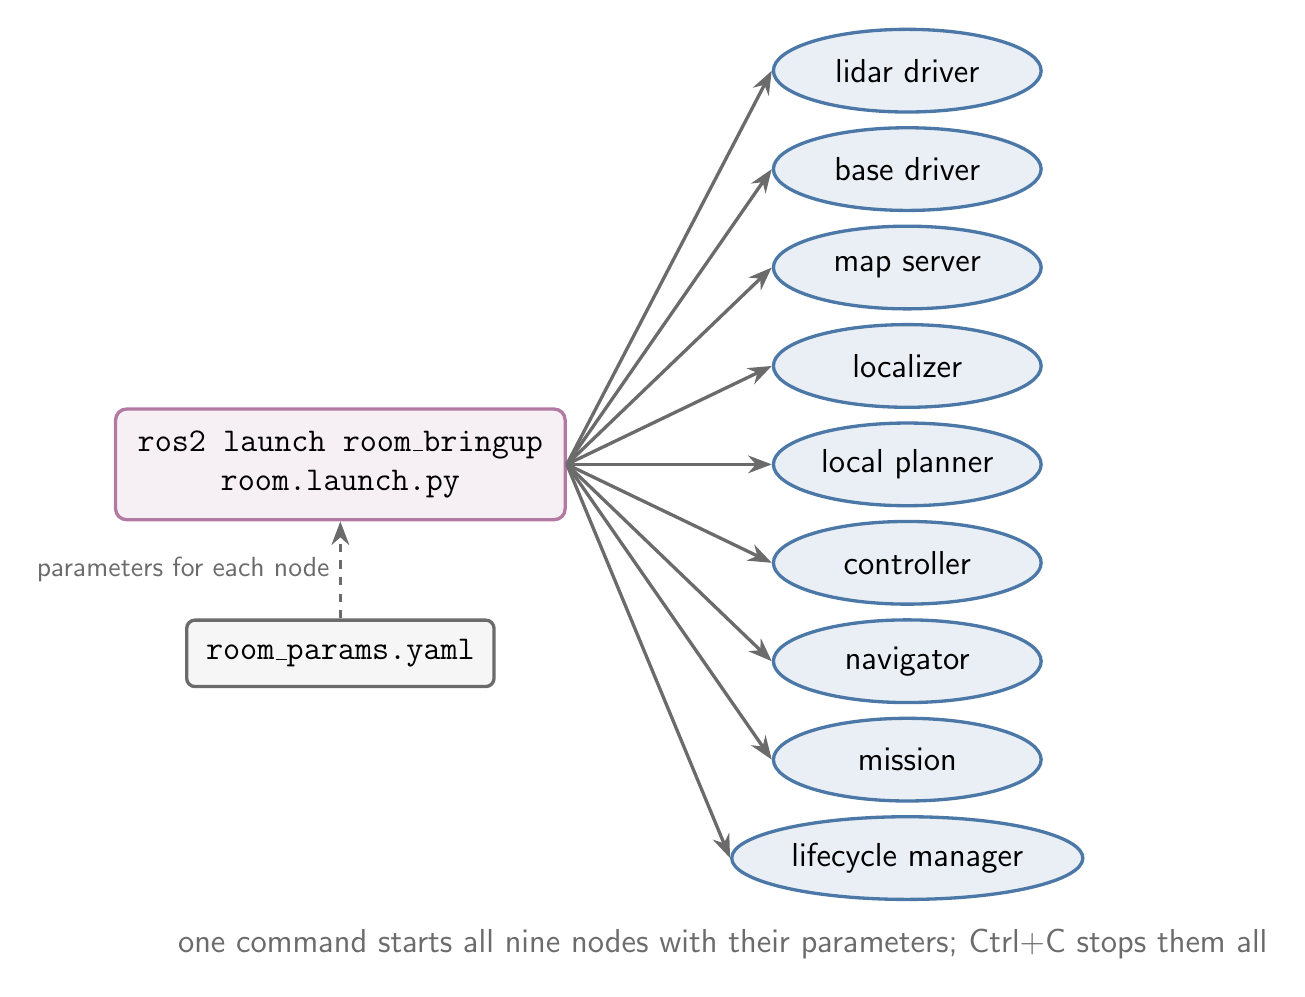
\begin{tikzpicture}[
  nd/.style={draw=cblue, fill=cblue!12, ellipse, font=\sffamily\large, inner sep=3pt, minimum width=3.4cm, minimum height=1.05cm},
  lf/.style={draw=cpurple, fill=cpurple!12, rounded corners=4pt, font=\ttfamily\large, align=center, inner sep=8pt},
  ar/.style={-{Stealth[length=3mm]}, draw=cgrey, line width=1.2pt}]
  \node[lf] (cmd) at (0,0) {ros2 launch room\_bringup\\ room.launch.py};
  \node[draw=cgrey, fill=cgrey!6, rounded corners=3pt, font=\ttfamily\large, inner sep=7pt] (par) at (0,-2.4) {room\_params.yaml};
  \foreach \n/\y in {lidar driver/5.0, base driver/3.75, map server/2.5, localizer/1.25, local planner/0, controller/-1.25, navigator/-2.5, mission/-3.75, lifecycle manager/-5.0}
    {\node[nd] (\n) at (7.2,\y) {\n}; \draw[ar] (cmd.east) -- (\n.west);}
  \draw[ar, dashed] (par.north) -- node[note, left, font=\sffamily\normalsize] {parameters for each node} (cmd.south);
  \node[note, font=\sffamily\large, align=left, anchor=west] at (-2.2,-6.1) {one command starts all nine nodes with their parameters; Ctrl+C stops them all};
\end{tikzpicture}
\end{document}
